\documentclass[%
 reprint,
%superscriptaddress,
%groupedaddress,
%unsortedaddress,
%runinaddress,
%frontmatterverbose, 
%preprint,
%showpacs,preprintnumbers,
%nofootinbib,
%nobibnotes,
%bibnotes,
 amsmath,amssymb,
 aps,
%pra,
%prb,
%rmp,
%prstab,
%prstper,
%floatfix,
]{revtex4-1}

\usepackage{graphicx}% Include figure files
\usepackage{dcolumn}% Align table columns on decimal point
\usepackage{bm}% bold math
%\usepackage{hyperref}% add hypertext capabilities
%\usepackage[mathlines]{lineno}% Enable numbering of text and display math
%\linenumbers\relax % Commence numbering lines

%\usepackage[showframe,%Uncomment any one of the following lines to test 
%%scale=0.7, marginratio={1:1, 2:3}, ignoreall,% default settings
%%text={7in,10in},centering,
%%margin=1.5in,
%%total={6.5in,8.75in}, top=1.2in, left=0.9in, includefoot,
%%height=10in,a5paper,hmargin={3cm,0.8in},
%]{geometry}

\usepackage{cmap} % Поиск в PDF
\usepackage[T2A]{fontenc} % Кодировка
\usepackage[utf8]{inputenc} % Кодировка исходного текста
\usepackage[english, russian]{babel} % Локализация и переносы
\frenchspacing % Более тонкая настройка пробелов 
\usepackage{multirow}
\usepackage[warn]{mathtext}
\usepackage{amssymb}
\usepackage{ dsfont }

% Переопределение англоязычного начертания каппа, фи и эпсилон, 
% а также знаков сравнения
\renewcommand{\epsilon}{\ensuremath{\varepsilon}}
\renewcommand{\phi}{\ensuremath{\varphi}} 
\renewcommand{\kappa}{\ensuremath{\varkappa}}
\renewcommand{\le}{\ensuremath{\leslant}}
\renewcommand{\leq}{\ensuremath{\leqslant}}
\renewcommand{\ge}{\ensuremath{\geslant}}
\renewcommand{\geq}{\ensuremath{\geqslant}}
\renewcommand{\emptyset}{\ensuremath{\varnothing}}

\usepackage{textcomp} 
\usepackage{indentfirst} % Красная строка
\usepackage{amsmath} % Текст в формулах
\usepackage{graphicx} % Графика
\DeclareGraphicsExtensions{.pdf,.png,.jpg}
\usepackage{pgfplots}
\pgfplotsset{compat=1.13}

%\usepackage{times}

\begin{document}

\title{Релаксационные колебания}
\thanks{3.5.3}

\author{Иван Едигарьев,}
\affiliation{
 Московский Физико-Технический Институт\\
 Факультет Общей и Прикладной Физики, 526т\\
}
%\date{\today}

\begin{abstract}
В работе предлагается снять вольт-амперную характеристику стабилитрона и познакомиться с работой релаксационного генератора: определить критическое сопротивление, исследовать зависимость периода колебаний от сопротивления при фиксированной ёмкости и от ёмкости при фиксированном сопротивлении.\\

В работе используются: стабилитрон СГ-2 (газонаполненный диод) на монтажной панели, амперметр, вольтметр, магазин сопротивлений, магазин емкостей, источник питания, осциллограф (ЭО), генератор звуковой частоты (ЗГ).\\

\end{abstract}

\pacs{Valid PACS appear here}% PACS, the Physics and Astronomy
                             % Classification Scheme.
%\keywords{Suggested keywords}%Use showkeys class option if keyword
                              %display desired
\maketitle

%\tableofcontent

\section{\label{sec:level1}Задание}

\subsection{\label{sec:level2}Характеристика стабилитрона}

1. Соберите схему, изображённую на рис. 1; к выходу источника питания подключите вольтметр (мультиметр СБМ), второй мультиметр используйте как амперметр. Правила работы с мультиметрами изложены в техническом описании (ТО) в конце папки.

Добавочное сопротивление $r$ подпаяно между ножкой лампы и соответствующей клеммой для того, чтобы предохранить стабилитрон от перегорания. Это сопротивление остаётся включённым при всех измерениях. Запишите величину $r$, указанную на панели лампы.

2. Установите регулятор источника питания на минимум напряжения и включите источник в сеть.

3. Снимите вольтамперную характеристику стабилитрона с резистором $r$ при возрастании и убывании напряжения. При этом как можно точнее определите потенциалы зажигания и гашения $V_1$ и $V_2$ и соответствующие токи $I_1$ и $I_2$.
\begin{center}
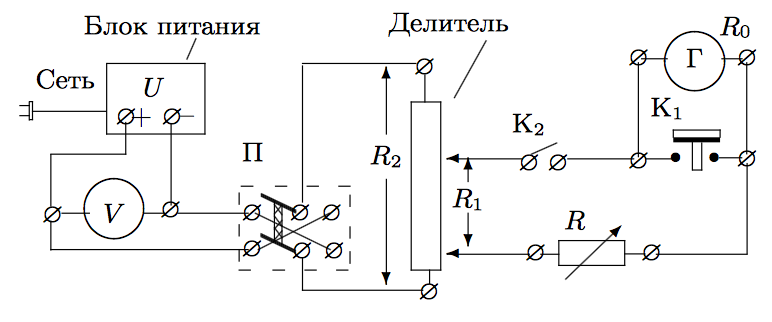
\includegraphics[scale = 0.35]{pic1.png}
\end{center}
\subsection{\label{sec:level2}Осциллограммы релаксационных колебаний}

4. Соберите релаксационный генератор согласно~рис. 2.

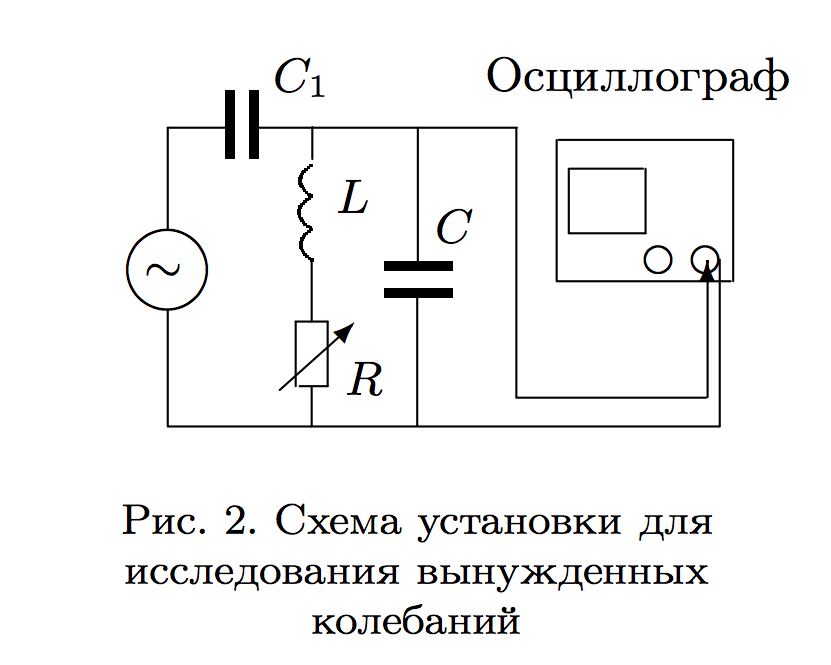
\includegraphics[scale = 0.22]{pic2.png}


5. Установите на магазине емкостей значение $C = 0,05$~мкФ, а на магазине сопротивлений	$R = 900$~кОм.

6. Включите в сеть звуковой генератор и источник питания; установите напряжение $U \simeq 1,2V_1$ (целое значение, близкое к рассчитанному).

7. Настройте осциллограф, руководствуясь техническим описанием, расположенным на установке.

Подберите частоту развёртки ЭО, при которой на экране видна картина пилообразных колебаний.

Если возникли трудности, сначала найдите колебания визуально. Для этого, сохранив $R = 900$~кОм, увеличьте ёмкость на порядок ($C = n \cdot 10^{-1}$~мкФ).При
таких больших значениях $R$ и $C$ возникают колебания с периодом в несколько секунд. Этот режим удобно использовать для проверки работоспособности собранного генератора. Если колебания видны глазом, можно искать пилу на экране, предварительно уменьшив ёмкость до величины $С = 0,05$~мкФ.

8. Получив пилу на экране, оцените соотношение между временем зарядки $\tau_{\text{з}}$ и временем разрядки $\tau_{\text{р}}$. Зарисуйте в тетрадь картину колебаний.

9. Уменьшая сопротивление магазина, определите при котором пропадают колебания, и сравните его с величиной, рассчитанной по формуле

\begin{equation}\label{1}
    R_{\text{кр}} = \frac{U - V_2}{I_2}. 
\end{equation}

Это сравнение полезно сделать в процессе работы и подумать о причинах расхождения результатов.

Убедитесь, что колебания пропадают не только при уменьшении $R$ при постоянном $U$, но и при увеличении $U$ при постоянном $R$, когда это $R$ не слишком превышает $R_{\text{кр}}$.

\subsection{\label{sec:level2}Фигуры Лиссажу и частота колебаний}

10. Восстановите исходные параметры релаксационного генератора: $C = 5 \cdot 10^{-2}$~мкФ, $R = 900$~кОм, $U \simeq 1,2V_1$.

Подайте сигнал с генератора на вход $X$ осциллографа.

Меняя частоту ЗГ, получите на экране фигуру Лиссажу без самопересечений, соответствующую отношению частот 1:1 (при сложении двух гармонических колебаний это был бы эллипс).

11. Не меняя параметров релаксационного генератора, уменьшите частоту ЗГ вдвое (втрое) и получите фигуры Лиссажу при соотношении частот 2:1 (3:1). Зарисуйте эти кривые в тетрадь (качественно).

Получите и зарисуйте фигуры Лиссажу при увеличении частоты ЗГ в два и три раза (1:2 и 1:3).

12. При любом целом значении $R$ из интервала $(2-4)~R_{\text{кр}}$ снимите с помощью фигур Лиссажу 1:1 зависимость частоты колебаний от ёмкости $C$, меняя величину ёмкости в пределах от $5 \cdot 10^{-2}$~до~$5 \cdot 10^{-3}$~мкФ.

Напряжение $U$, необходимое для расчёта теоретического значения периода по формуле
$$ T \approx \tau_{\text{з}} = RC \ln {\frac{U - V_2}{U - V_1}},$$
следует поддерживать постоянным.

13. Проведите серию измерений $\nu = f(R)$ при постоянной ёмкости $5 \cdot 10^{-2}$ мкФ, меняя величину $R$ от максимального значения до критического.

\begin{center}
Обработка результатов
\end{center}
1. Постройте графики $I = f(V)$ для системы, состоящей из стабилитрона и дополнительного сопротивления $r$ (по результатам измерений) и для стабилитрона без сопротивления $r$ (вычитая падение напряжения на сопротивлении $r$ при каждом токе). Сравните относительные изменения тока и напряжения на стабилитроне.\\
2. Рассчитав экспериментальные и теоретические значения периодов, постройте графики $T_{\text{эксп}}~=~f(C)$ и $T_{\text{теор}}~=~f(C)$ на одном листе.\\
3. На другом листе постройте графики $T_{\text{эксп}}~=~f(R)$ и $T_{\text{теор}}~=~f(R)$.\\
4. Если наклоны теоретической и экспериментальной прямых заметно отличаются, рассчитайте из экспериментальной прямой динамический потенциал гашения. Потенциалы зажигания можно считать одинаковыми.

\subsection{\label{sec:level2}Данные}

Построим график зависимости $I = f(V)$ для системы, состоящей из стабилитрона и дополнительного сопротивления $r$ (График 1) и для стабилитрона без сопротивления $r$ (График 2):\\
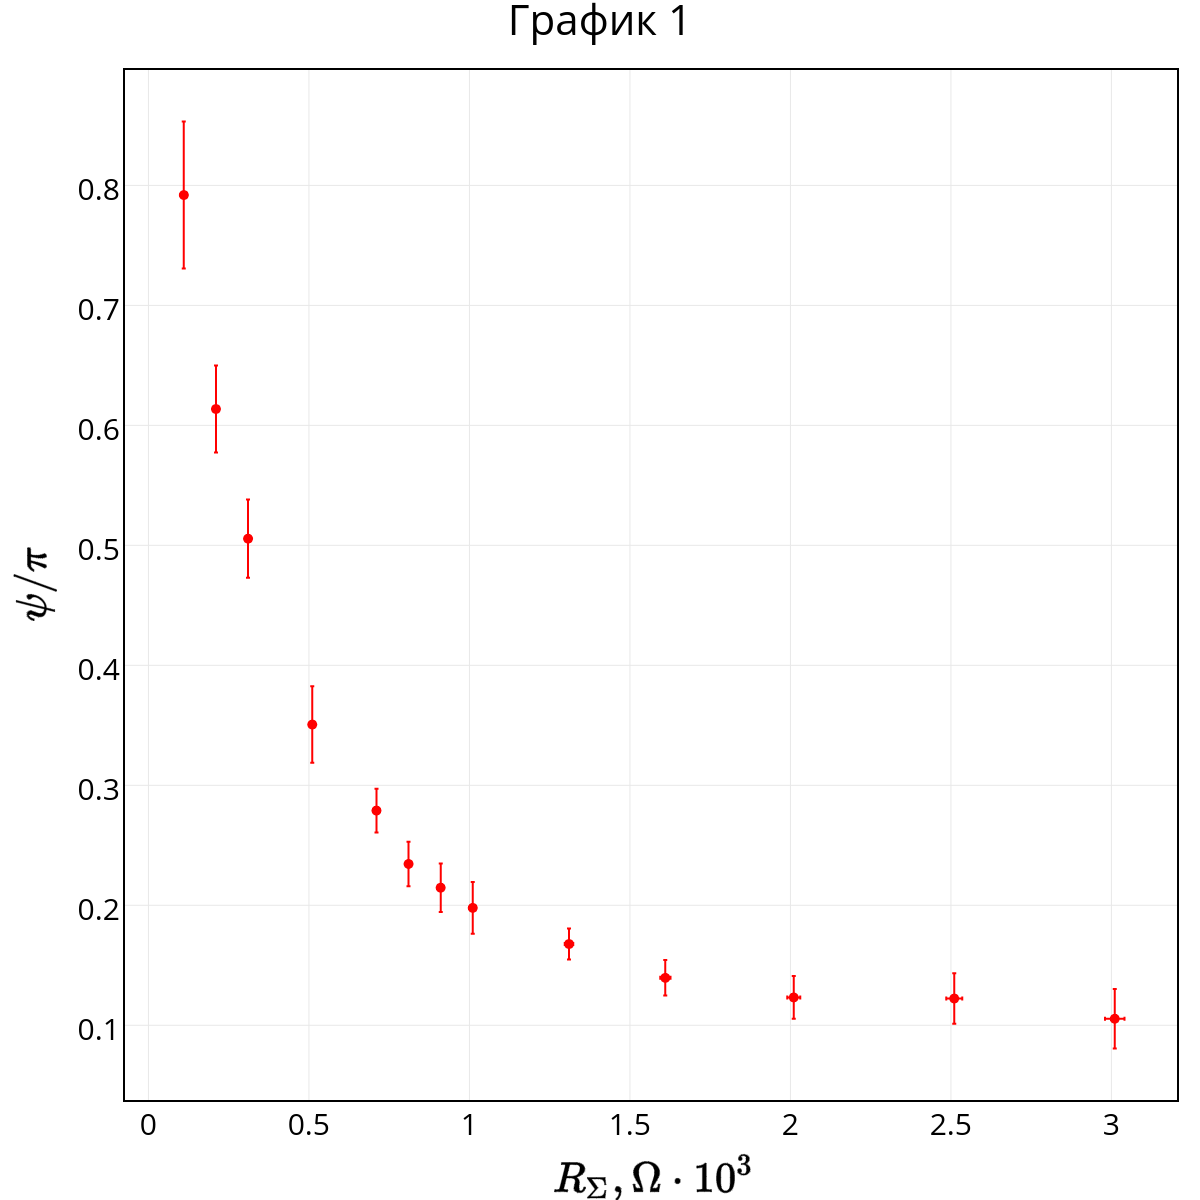
\includegraphics[scale = 0.19]{my_plot1.png} \\
\\
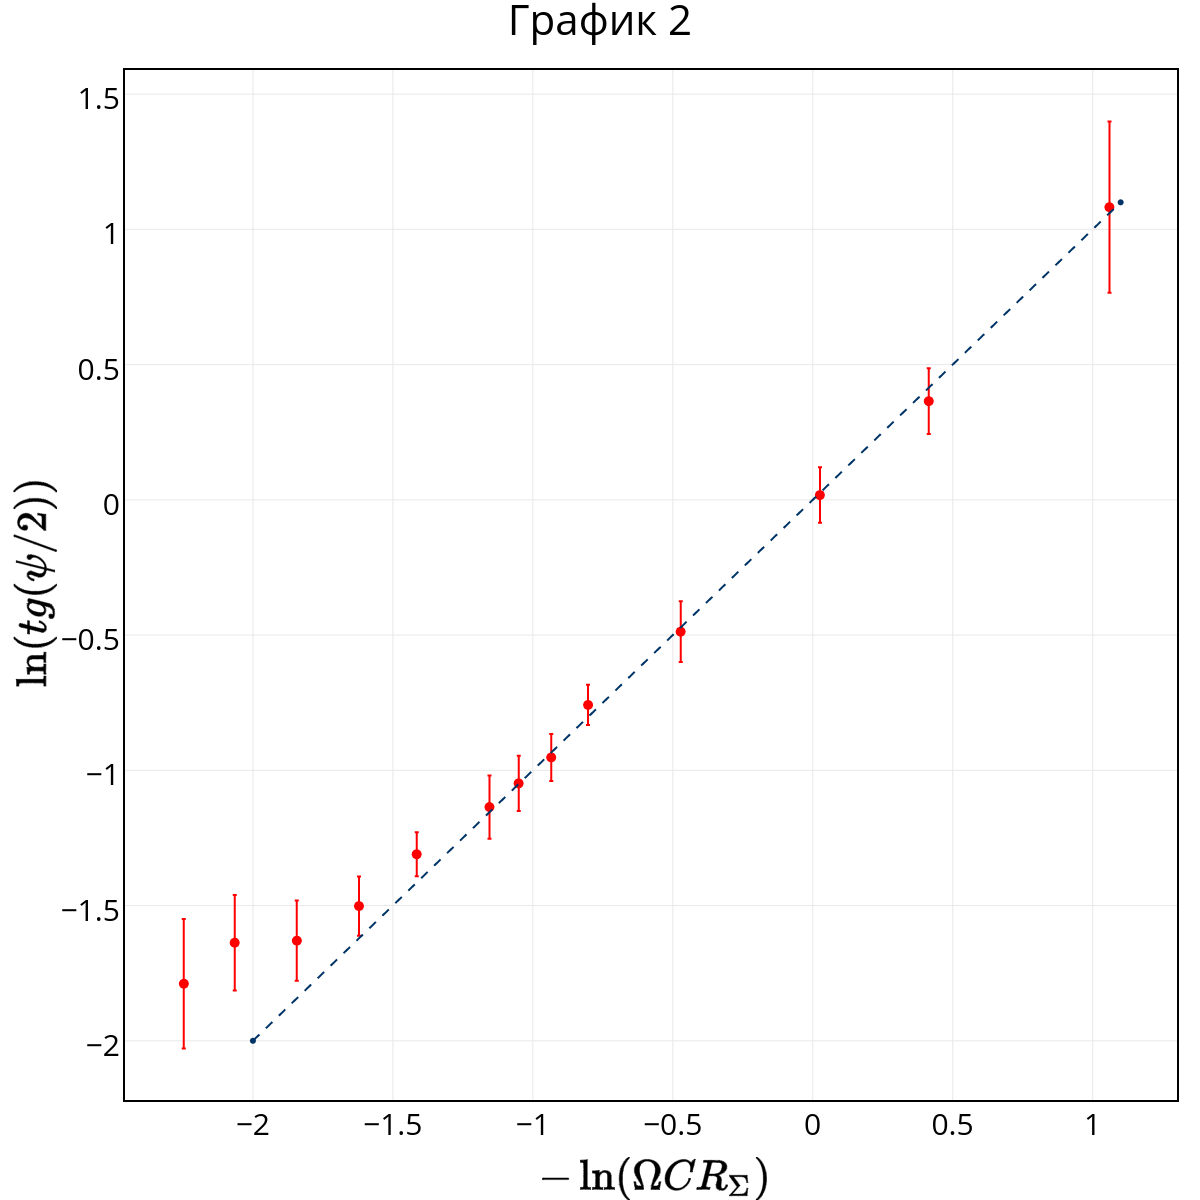
\includegraphics[scale = 0.19]{my_plot2.png}

В момент гашения стабилитрона ток в цепи падал до значение порядка $10^{-5}$ A, что вызывало уменьшение падающего на сопротивление напряжения и, следовательно, увеличение напряжения на стабилитроне. Не будем использовать значения, измеренные в выключенном состоянии, а возьмём ближайшие к ним. Получим данные параметры:
$$\boxed{V_1^{\text{exp}} = 85.6~V,~~~I_1^{\text{exp}} = 2.7 \cdot 10^{-3}~A}$$
$$V_2^{\text{exp}} = 75.1~V,~~~I_2^{\text{exp}} = 1.2 \cdot 10^{-3}~A$$

Во время работы с помощью осциллографа была сделана оценка на время зарядки $\tau_{\text{з}}$ и разрядки $\tau_{\text{р}}$:
$$\tau_{\text{з}} = 29~\text{дел},~~\tau_{\text{р}} = 2~\text{дел}$$

Отношение данных времён позволяет нам в дальнейшем пренебречь временем разрядки по сравнению с временем зарядки.

Во время работы согласно методическому описанию было проведено измерение сопротивления, при котором пропадают колебания, и сравнение с сопротивлением, рассчитанным по формуле (1) с помощью потенциалов и токов гашения и зажигания. Данные измерения плохо согласуются и можно говорить о расхождении результатов на данном этапе (см. Выполнение). Стоит заметить, что при этом можно выделить линейную зависимость ошибки от значения падающего напряжения.

Далее рассчитаем экспериментальные и теоретические значения периодов колебаний и построим графики $T_{\text{эксп}} = f(C)$ и $T_{\text{теор}} = f(C)$ (График 3).\\
\\
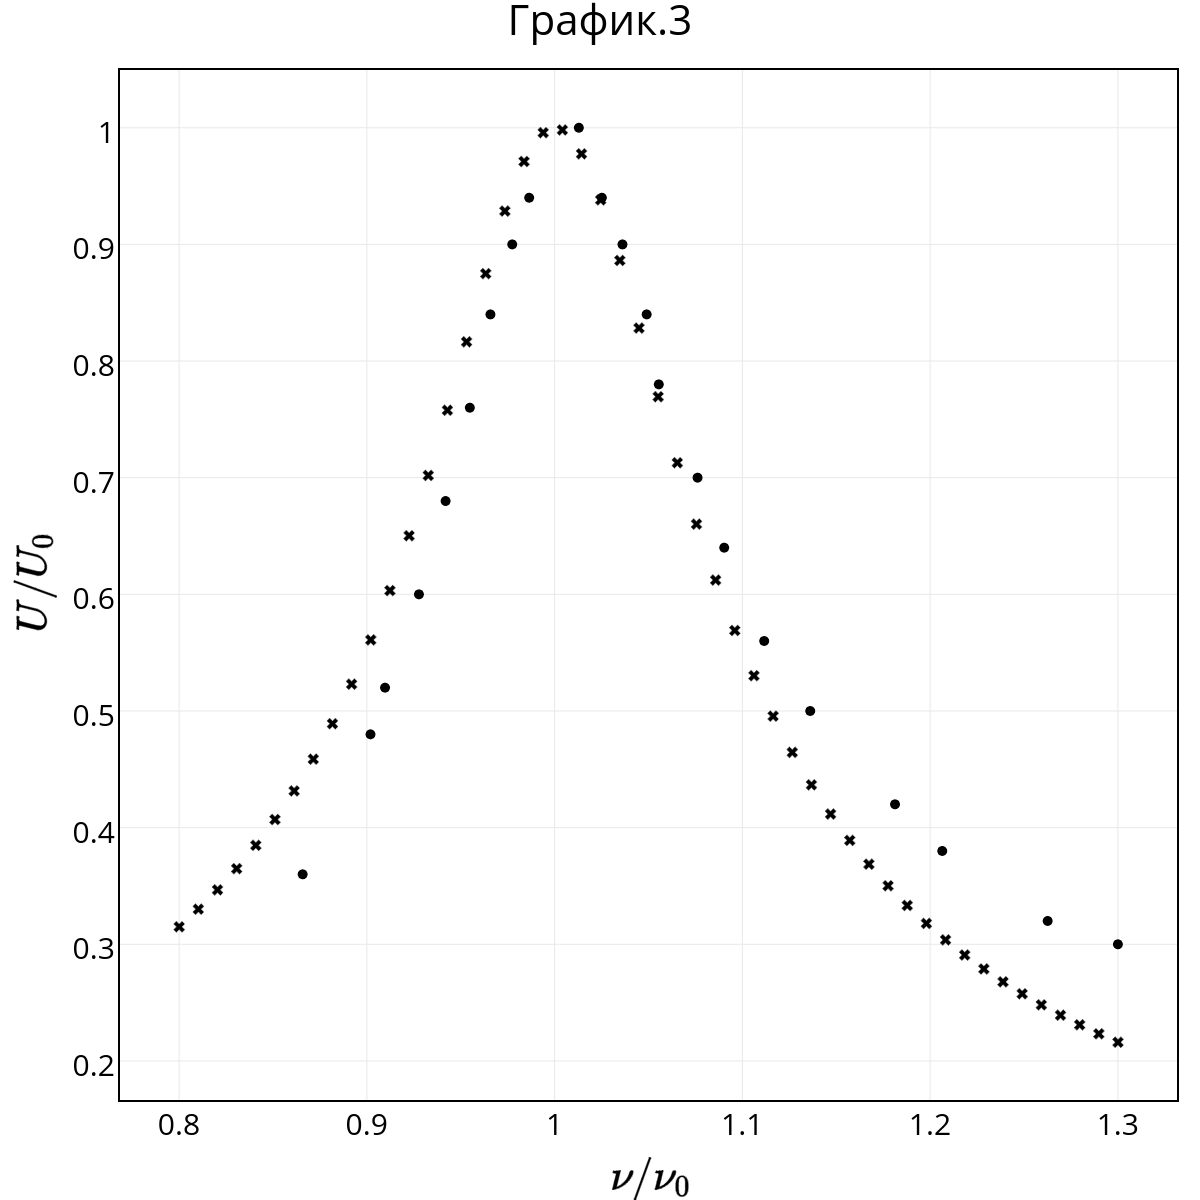
\includegraphics[scale = 0.19]{my_plot3.png}\\
\\
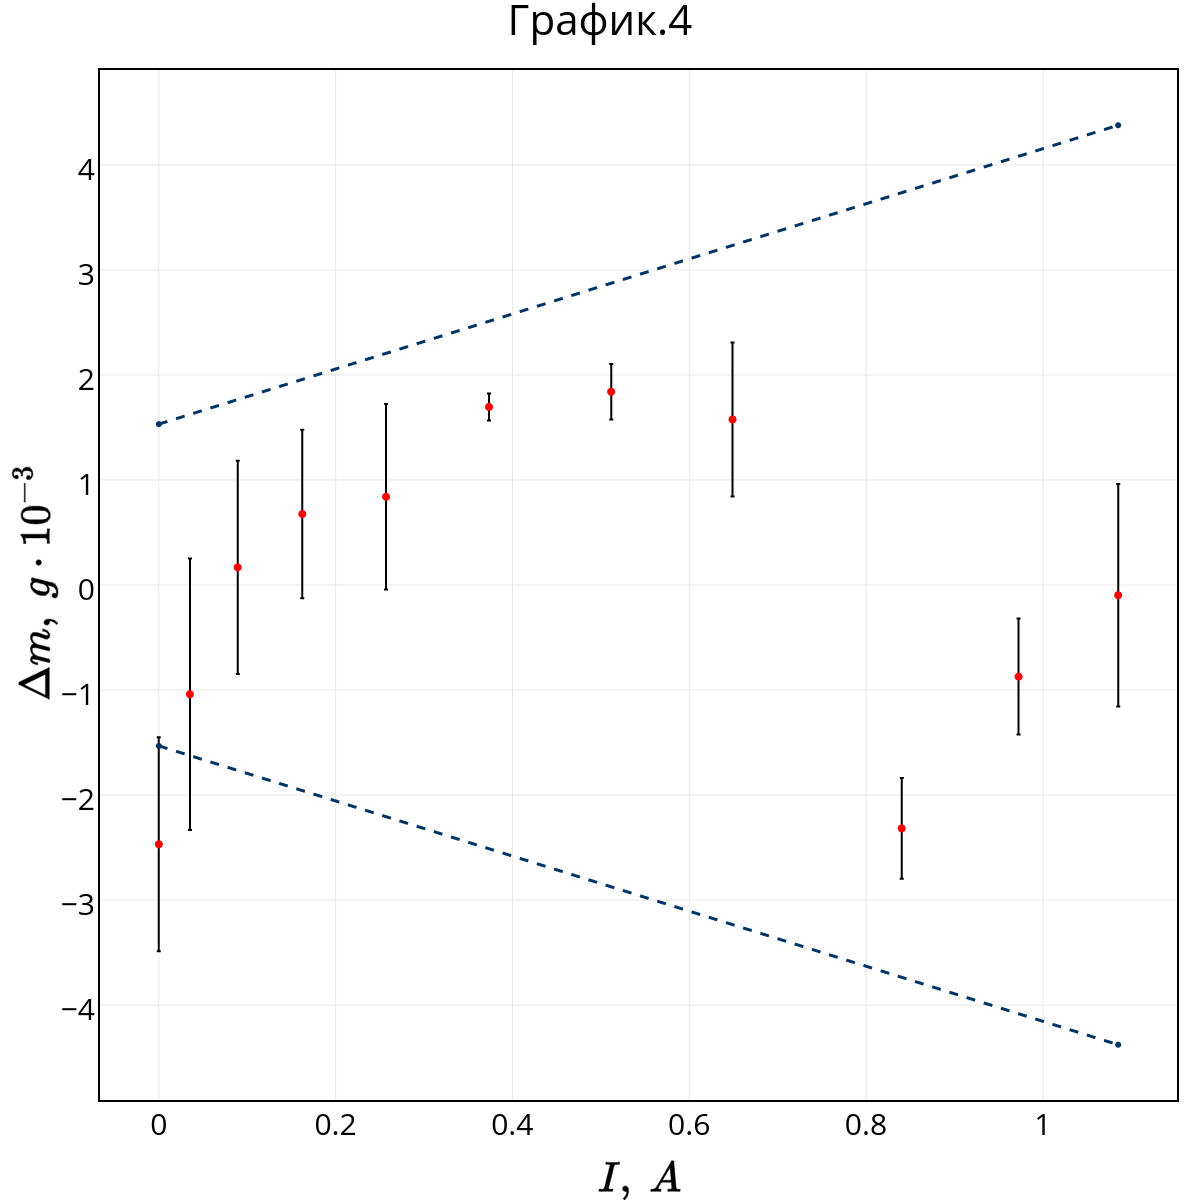
\includegraphics[scale = 0.19]{my_plot4.png}\\

Аналогично поступим и с зависимостями $T_{\text{эксп}}~=~f(R)$ и $T_{\text{теор}} = f(R)$ (График 4).\\

Заметим, что существует достаточно большое расхождение с теорией в обеих зависимостях. Рассчитаем из экспериментальной прямой динамический потенциал гашения, построим линейную регрессию вида $f(x) = \beta x$ с квадратичной функцией потерь. Получим:
$$\text{для}~f(C):~ \ln {\frac{U - V_2^{\text{C}}}{U - V_1^{\text{C}}}} = 1.13 \pm 0.04^{\text{stat}}$$
$$\text{для}~f(R):~ \ln {\frac{U - V_2^{\text{R}}}{U - V_1^{\text{R}}}} = 1.11 \pm 0.03^{\text{stat}}$$

Вычислим новые значения для потенциала гашения, измеренные через изменения $C$ и $R$:
$$\boxed{V_2^{\text{C}} = 43 \pm 2^{\text{stat}}~V}$$
$$\boxed{V_2^{\text{R}} = 44 \pm 2^{\text{stat}}~V}$$

Вычитая падение напряжения на сопротивление и усредняя данные по двум опытам, получим итоговый ответ и оценим ошибку:
$$\boxed{V^{\text{заж}} = (71 \pm 3^{\text{syst}})~V,~~~I^{\text{заж}} = (2.7 \pm 0.1^{\text{stat}}) \cdot 10^{-3}~A}$$
$$\boxed{V^{\text{гаш}} = (37 \pm 2^{\text{stat}} \pm 2^{\text{syst}} )~V,~~~I^{\text{гаш}} = (1.2 \pm 0.1^{\text{stat}}) \cdot 10^{-3}~A}$$

Картину релаксационных колебаний и качественную зарисовку фигур Лисажу можно найти в приложении к данной работе, в пунктах 1) и 2) соответственно.

\end{document}